% Preamble
% ---
\documentclass{article}

% Packages

% \usepackage{graphicx}
% \usepackage{subfig}

\usepackage{multicol}
\usepackage{float}

\usepackage{tikz}
\usepackage{pgfplots}
\usepgfplotslibrary{external}
% \usetikzlibrary{shapes.geometric, arrows}
% 
\usepackage[english]{babel}
\usepackage{hyperref} % 1 -> Figure 1
\usepackage{caption}

% code block
\usepackage{xcolor}
\usepackage{listings}

% tikz
\usetikzlibrary{arrows.meta}

\definecolor{mGreen}{rgb}{0,0.6,0}
\definecolor{mGray}{rgb}{0.5,0.5,0.5}
\definecolor{mPurple}{rgb}{0.58,0,0.82}
\definecolor{backgroundColour}{rgb}{0.95,0.95,0.92}

\lstdefinestyle{CStyle}{
    backgroundcolor=\color{backgroundColour},   
    commentstyle=\color{mGreen},
    keywordstyle=\color{magenta},
    numberstyle=\tiny\color{mGray},
    stringstyle=\color{mPurple},
    basicstyle=\footnotesize,
    breakatwhitespace=false,         
    breaklines=true,                 
    captionpos=b,                    
    keepspaces=true,                 
    numbers=left,                    
    numbersep=2pt,                  
    showspaces=false,                
    showstringspaces=false,
    showtabs=false,                  
    tabsize=2,
    language=C
}

\pgfplotscreateplotcyclelist{mylist}{%
red,every mark/.append style={fill=red!80!black},mark=*,mark size=3pt\\%
brown!60!black,every mark/.append style={fill=brown!80!black},mark=*, mark size=3pt\\%
black,every mark/.append style={fill=black!80!black},mark=*, mark size = 3pt\\%
}


\usepackage{geometry}
\geometry{margin=1.2cm}

\title{Optimisation of d2q9-bgk Lattice Boltzmann Scheme with MPI}
\author{James Elgar, za18968}
\date{\today}

\begin{document}
\begin{multicols}{2}

\maketitle

\section{Introduction}

This report will explore the use of distributed memory parallelism to optimize
a given algorithm. The algorithm solves a d2q9-bgk Lattice Boltzmann scheme
over a grid of cells. The report will evaluate different approaches to
distributed memory parallelism, mostly using the Message Parsing Interface,
MPI, standard. When optimizing a distributed memory problem there are various
factor which can effect the performance of the algorithm. This report will
focus of the optimization of individual nodes, the data layout of the cells
array, the use of blocking vs non-blocking sends and final compare the use of
MPI for running with multiple processor with OpenCL for running with a graphics
card.

\section{MPI}

In this MPI implementation 4 nodes were used. In order to distribute the work
across these 4 different nodes, the grid is divided up into 4 sections. When
dividing a grid into different sections there are generally 2 approaches, in
square sub grids or in rows (or columns). \autoref{fig:dist-tiled} is an example of splitting a grid up as a set of square subsection. This approach 
and \autoref{fig:dist-rows}

\begin{center}
\begin{multicols}{2}

% Tiles
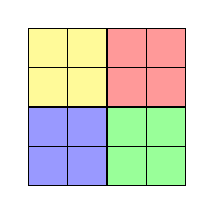
\begin{tikzpicture}[every node/.style={minimum size=.5cm-\pgflinewidth, outer sep=0pt}, scale=0.5]
    \fill[blue!40!white] (0,0) rectangle (2,2);
    \fill[red!40!white] (2,2) rectangle (4,4);
    \fill[green!40!white] (2,0) rectangle (4,2);
    \fill[yellow!40!white] (0,2) rectangle (2,4);
    \draw[step=1cm,color=black] (0,0) grid (4,4);
\end{tikzpicture}
\captionof{figure}{Tiled distribution}
\label{fig:dist-tiled}

% Rows 
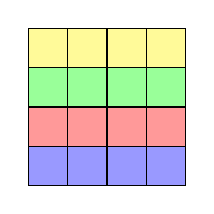
\begin{tikzpicture}[every node/.style={minimum size=.5cm-\pgflinewidth, outer sep=0pt}, scale=0.5]
    \fill[blue!40!white] (0,0) rectangle (4,1);
    \fill[red!40!white] (0,1) rectangle (4,2);
    \fill[green!40!white] (0,2) rectangle (4,3);
    \fill[yellow!40!white] (0,3) rectangle (4,4);
    \draw[step=1cm,color=black] (0,0) grid (4,4);
\end{tikzpicture}
\captionof{figure}{Rows distribution}
\label{fig:dist-rows}

\end{multicols}
\end{center}

% Halo regions

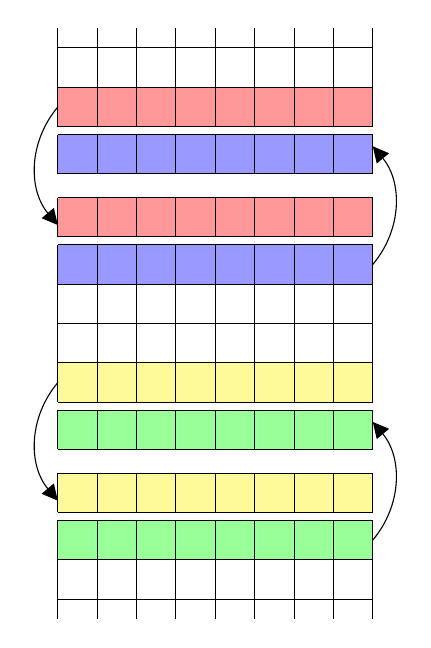
\begin{tikzpicture}[every node/.style={minimum size=.5cm-\pgflinewidth, outer sep=0pt}, scale=0.5]
    \fill[red!40!white, yshift=1cm] (0,6) rectangle (8,7);
    \draw[step=1cm,color=black,yshift=1cm] (0,6) grid (8,8.5);

    % Blue Halo
    % \node[main node] (1) {a};
    \fill[blue!40!white, yshift=-0.2cm] (0,6) rectangle (8,7);
    \draw[step=1cm,color=black,yshift=-0.2cm] (0,6) grid (8,7);

    % Red Halo
    \fill[red!40!white, yshift=0.2cm] (0,4) rectangle (8,5);
    \draw[step=1cm,color=black,yshift=0.2cm] (0,4) grid (8,5);

    % \node[] (BR) at (8, 3.5) {};
    \fill[blue!40!white] (0,3) rectangle (8,4);
    \fill[yellow!40!white] (0,0) rectangle (8,1);
    \draw[step=1cm,color=black] (0,0) grid (8,4);

    % Green Halo
    \fill[green!40!white, yshift=-0.2cm] (0,0) rectangle (8,-1);
    \draw[step=1cm,color=black,yshift=-0.2cm] (0,0) grid (8,-1);
    
    % Yellow Halo
    \fill[yellow!40!white, yshift=0.2cm] (0,-2) rectangle (8,-3);
    \draw[step=1cm,color=black,yshift=0.2cm] (0,-2) grid (8,-3);

    \fill[green!40!white, yshift=-1cm] (0,-2) rectangle (8,-3);
    \draw[step=1cm,color=black,yshift=-1cm] (0,-2) grid (8,-4.5);

    % Arrows
    \draw [-{Triangle[length=2mm, width=2mm]}] (8, +3.5) to [bend right=40] (8, +6.5);
    \draw [-{Triangle[length=2mm, width=2mm]}] (0, +7.5) to [bend right=40] (0, +4.5);
    \draw [-{Triangle[length=2mm, width=2mm]}] (0, +0.5) to [bend right=40] (0, -2.5);
    \draw [-{Triangle[length=2mm, width=2mm]}] (8, -3.5) to [bend right=40] (8, -0.5);

\end{tikzpicture}
\captionof{figure}{Cell regions and halos}
\label{fig:cells-regions-and-halos}

The provided algorithm was optimised using shared memory parallelism with
OpenMP. This means every every thread has access to the same region of memory
which is manipulated during the calculations. When migrating a program to use
distributed memory the important consideration is what memory is required by
each node.

% Inital implementation blocking send
% Data shape to reduce number of sends

\section{SOA vs AOS}

% Switching to AOS to ensure contigious data sends 

\section{OpenMP MPI}

% Combining shared memory and distributed memory parallelism

\section{Non-Blocking Send}

\section{OpenCL}

\end{multicols}
\end{document}
